%!TEX encoding = UTF-8 Unicode
% ================================================================================
\documentclass[
    fontsize=12pt,
    headings=small,
    parskip=half,           % Ersetzt manuelles Setzen von parskip/parindent.
    bibliography=totoc,
    numbers=noenddot,       % Entfernt den letzten Punkt der Kapitelnummern.
    open=any,               % Kapitel kann auf jeder Seite beginnen.
%   final                   % Entfernt alle todonotes und den Entwurfstempel.
    ]{scrreprt}
% ===================================Praeambel==================================
%!TEX encoding = UTF-8 Unicode
%!TEX root = hinweiseabschlussarbeit.tex

% Kodierung, Sprache, Patches {{{
\usepackage[T1]{fontenc}    % Ausgabekodierung; ermöglicht Akzente und Umlaute
                            %  sowie korrekte Silbentrennung.
\usepackage[utf8]{inputenc} % Erlaubt die direkte Eingabe spezieller Zeichen;
                            %  utf8 muss die Eingabekodierung des Editors sein.
\usepackage[ngerman]{babel} % Deutsche Sprachanpassungen (z.B. Überschriften).
\usepackage{microtype}      % Optimale Randausrichtung und Skalierung.
\usepackage[
    autostyle,
    ]{csquotes}             % Korrekte Anführungszeichen in der Literaturliste.
%\usepackage{fixltx2e}      % Patches fuer LaTeX2e - seit 2015 nicht mehr nötig
\usepackage{scrhack}        % Verhindert Warnungen mit älteren Paketen.
\usepackage[
  newcommands
]{ragged2e}                 % Verbesserte \ragged...Befehle
\PassOptionsToPackage{
  hyphens
}{url}                      % Sorgt für URL-Umbrüche in Fußzeilen u. Literatur
% }}}

% Schriftarten {{{
\usepackage{mathptmx}       % Times; modifies the default serif and math fonts
\usepackage[scaled=.92]{helvet}% modifies the sans serif font
\usepackage{courier}        % modifies the monospace font
% }}}

% Biblatex {{{
\usepackage[
    style=alphabetic,
    backend=biber,
    %backref=true
    ]{biblatex}             % Biblatex mit alphabetischem Style und biber.
\bibliography{literaturliste.bib} % Dateiname der bib-Datei.
\DeclareFieldFormat*{title}{
    \mkbibemph{#1}}         % Make titles italics
% }}}

% Dokument- und Texteinstellungen {{{
\usepackage[
    a4paper,
    margin=2.54cm,
    marginparwidth=2.0cm,
    footskip=1.0cm
    ]{geometry}             % Ersetzt 'a4wide'.
\clubpenalty=10000          % Keine Einzelzeile am Beginn eines Absatzes
                            %  (Schusterjungen).
\widowpenalty=10000         % Keine Einzelzeile am Ende eines Absatzes
\displaywidowpenalty=10000  %  (Hurenkinder).
\usepackage{floatrow}       % Zentriert alle Floats
\usepackage{ifdraft}        % Ermöglicht \ifoptionfinal{true}{false}
\pagestyle{plain}           % keine Kopfzeilen
% \sloppy                    % großzügige Formatierungsweise
\deffootnote{1em}{1em}{
  \thefootnotemark.\ }      % Verbessert Layout mehrzeiliger Fußnoten
\ifdefined\chapterformat
	\renewcommand*{\chapterformat}{% Hübscht Kapitelüberschrift mit senkrechtem 
		\thechapter\enskip%          grauen Balken zwischen Nummer und Text auf
		\textcolor{gray!50}{\rule[-\dp\strutbox]{2pt}{\baselineskip}}\enskip
	}
\fi
%\setkomafont{disposition}{\normalcolor\bfseries} % Aus der KOMA-Skript-Anleitung: „Mit dieser Änderung verzichten Sie darauf, für alle Gliederungsebenen serifenlose Schrift voreinzustellen“

\makeatletter
\AtBeginDocument{%
    \hypersetup{%
        pdftitle = {\@title},
        pdfauthor  = \@author,
    }
}
\makeatother
% }}}

\newcommand*\rot[1]{\rotatebox{90}{#1}}

% Weitere Pakete {{{
\usepackage{graphicx}       % Einfügen von Graphiken.
\usepackage{tabu}           % Einfügen von Tabellen.
\usepackage{multirow}       % Tabellenzeilen zusammenfassen.
\usepackage{multicol}       % Tabellenspalten zusammenfassen.
\usepackage{booktabs}       % Schönere Tabellen (\toprule\midrule\bottomrule).
\usepackage[nocut]{thmbox}  % Theorembox bspw. für Angreifermodell.
\usepackage{amsmath}        % Erweiterte Handhabung mathematischer Formeln.
\usepackage{amssymb}        % Erweiterte mathematische Symbole.
\usepackage{rotating}
\usepackage{longtable}      % for 'longtable' environment
\usepackage{pdflscape}      % for 'landscape' environment
\usepackage{xltabular}
\usepackage[
    printonlyused
    ]{acronym}              % Abkürzungsverzeichnis
\usepackage[
    colorinlistoftodos,
    textsize=tiny,          % Notizen und TODOs - mit der todonotes.sty von
    \ifoptionfinal{disable}{}%  Benjamin Kellermann ist das Package "changebar"
    ]{todonotes}            %  bereits integriert.
\usepackage[
    breaklinks,
    hidelinks,
    pdfdisplaydoctitle,
    pdfpagemode = {UseOutlines},
    pdfpagelabels,
    ]{hyperref}             % Sprungmarken im PDF. Lädt das URL-Paket.
    \urlstyle{rm}           % Entfernt die Formattierung von URLs.
%\usepackage{breakurl}
%\def\UrlBreaks{\do\/\do-}
\usepackage{listings}       % Spezielle Umgebung für Quelltextformatierung.
    \lstset{                
        language=C,
        breaklines=true,
        breakatwhitespace=true,
        frame=l,            % Linie links: l, doppelt: L
		framerule=2.5pt,    % Dicke der Linie
		rulecolor=\color{gray},% Farbe der Linie
        captionpos=b,
        xleftmargin=6ex,
        tabsize=4,
        numbers=left,
        numberstyle=\ttfamily\footnotesize,
        basicstyle=\ttfamily\footnotesize,
        keywordstyle=\bfseries\color{green!50!black},
        commentstyle=\itshape\color{magenta!90!black},
        identifierstyle=\ttfamily,
        stringstyle=\color{orange!90!black},
        showstringspaces=false,
        }

\usepackage{algorithm}
\usepackage{algpseudocode}
%\usepackage{filecontents}  % Direktes Einfügen von Dateiinhalt. Wird hier für
                            %  die Verwendung einer .bib-Datei in dieser .tex-
                            %  Datei benötigt.
% }}}

% ===================================Dokument===================================

\title{Intrusion detection for OAuth}
\author{Florian Nehmer}
\date{06.01.2023} % Falls ein bestimmtes Datum eingesetzt werden soll, einfach
                    %  diese Zeile aktivieren.

\begin{document}

\begin{titlepage}% {{{
	
\includegraphics[width=6.8cm]{./pic/up-uhh-logo-u-2010-u-farbe-u-rgb.pdf}
	\begin{center}\Large
		\vfill
		Masterarbeit
		\vfill
		\makeatletter
		{\Large\textsf{\textbf{\@title}}\par}
		\makeatother
		\vfill
		vorgelegt von
		\par\bigskip
		\makeatletter
		{\@author} \par
		\makeatother
		Matrikelnummer 6417446 \par
		Studiengang Informatik
		\vfill
		MIN-Fakultät \par
		Fachbereich Informatik
		\vfill
		\makeatletter
		eingereicht am {\@date}
		\makeatother
		\vfill
		Betreuer: Pascal Wichmann, M.\,Sc. Informatik \par
		Erstgutachter: Prof. Dr.-Ing. Hannes Federrath \par
		Zweitgutachter: Pascal Wichmann, M.\,Sc. Informatik.
	\end{center}
	\ifoptionfinal{}{
	\begin{tikzpicture}[remember picture, overlay]
		\node[draw, red, font=\ttfamily\bfseries\Large, xshift=30mm, yshift=238mm,
			rotate=340, text centered, text width=6cm, very thick, rounded
			corners=4mm] at (current page.south) {Entwurf vom \today};
	\end{tikzpicture}
	% ====> Delete me
	\begin{tikzpicture}[overlay]
		\node[draw, blue, font=\sffamily\Large, xshift=0mm, yshift=210mm, rotate=0, text centered, rounded corners=1mm] at (current page.south) {Muster des Deckblatts für Abschlussarbeiten};
	\end{tikzpicture}
	% <==== /Delete me
	}
\end{titlepage}% }}}

\chapter*{Aufgabenstellung}
OAuth [RFC6749] is a widely used authentication protocol, which is typically used between multiple actors, such as different organizations. As authentication is at the core of application security, it is specifically essential to prevent attacks on the authentication.

The tasks of this thesis are as follows: Firstly, a systematic literature study should be performed on existing properties and attacks on the OAuth protocol or its implementations. Secondly, the thesis should design protection strategies for the threats that are not sufficiently solved in existing solutions. Two options for this step are (i) the utilization of anomaly-based intrusion detection for OAuth and (ii) specification-based intrusion detection for OAuth. Thirdly, the thesis should evaluate the security of the designed architecture and compare it to other solutions.

\chapter*{Zusammenfassung}

Für die eilige Leserin bzw. den eiligen Leser sollen auf etwa einer halben, maximal einer Seite die wichtigsten Inhalte, Erkenntnisse, Neuerungen bzw. Ergebnisse der Arbeit beschrieben werden.

Durch eine solche Zusammenfassung (im Engl. auch Abstract genannt) am Anfang der Arbeit wird die Arbeit deutlich aufgewertet. Hier sollte vermittelt werden, warum man die Arbeit lesen sollte.

\tableofcontents

\chapter{Introduction}
\label{chap.introduction}
\section{Motivation}
\section{Research Question}
\section{Outline}

\chapter{Fundamental Knowledge}
\label{chap.fundamental_knowledge}

\section{OAuth 2.0 protocol}
The Open Authorization 2.0 protocol nowadays often referred to as the \emph{OAuth} protocol, is an authorization framework, that allows third-party applications to gain limited access to resources in a different location on behalf of the party, that owns these resources. For many users of the Internet, it is in practice the protocol behind the ``\emph{Sign in with ...}'' button. The current standard, first defined in 2012 in RFC6749, is already the successor of the OAuth 1.0 standard, which was officially published in 2010 by the IETF in RFC5849 \cite{hammer2010rfc}. In the meantime, several extensions for the protocol were published as standards and technical reports. These extensions include new functionalities for the protocol e.g. the ability to use the protocol with devices like smart TVs and printers \cite{denniss2019oauth} or documents, which describe several security considerations when implementing the protocol in practice \cite{lodderstedt2020oauth}.

The current version of the OAuth protocol grew over time and nowadays has many involved actors and offers several different modes of operation.

\subsection{Involved actors}
In general, there are four involved actors in the OAuth protocol:
\begin{itemize}
	\item Resource owner: 
	The resource owner is the entity that owns or is allowed to manage protected resources. The resource owner might grant access to these resources.
	\item Resource server: The resource server is the server, where the protected resources are stored. It can accept or decline authorization tokens, which it receives from the client.
	\item Client: The client is an entity, which makes requests to get access to the protected resources, on behalf of the resource owner.
	\item Authorization server: The server, that manages access to the protected data. It issues access tokens to the client after successful authentication of the resource owner.
\end{itemize}

Depending on the protocol mode, these four actors exchange different messages in variable ways. 

\subsection{Front-channel and Back-channel messages}

Regarding security considerations messages are categorized into two main categories, \emph{front-channel} and \emph{back-channel}. As the protocol is mostly used in the application layer using HTTP and TLS, \emph{front-channel} means that the message is transported via the \emph{Request-URI} \cite[Sec. 5.1.2]{fielding1999hypertext} e.g. by using query parameters. An attacker, which is able to eavesdrop on network traffic would be able to read such messages.
\emph{Back-channel} means on the other hand that the message is transported via the HTTP message body. In the case of HTTPS, this means the attacker, who eavesdrops on the network traffic is not able to read the message anymore, as it is encrypted. 

\subsection{Grant Types}
The protocol flow is dependent on the protocol mode. In the case of OAuth the different protocol modes are called \emph{Grant types}, as the modes differ on how the authorization is granted to the resource owner via the client.
\todo{write about general OAuth flow with graphic, see rfc}

\subsubsection{Authorization Code Grant}
According to a recent study, the authorization code grant mode of OAuth is the most used protocol mode for OAuth on the internet \cite[Table 1]{philippaerts2022oauch}. It is offered by more than 90\% of all identity providers.

In this mode illustrated in Figure 2.1, a resource owner aiming to access protected data via a REST API utilizes a user agent, in this case a web browser, to interact with a client application that manages API requests through the user agent.
The process begins as the client redirects the user agent to the authorization server through the front channel. The message contains a client ID, a redirect URL and a state. The client ID is a unique identifier of the protected resource. The redirect URI is the location the user agent is redirected to after authentication. The state can hold any string value and is most commonly used for CSRF tokens. 
The authorization server now asks the resource owner for authentication. If the resource owner is authenticated and is allowed to access the desired protected resources, the user agent gets redirected back using the redirect URI. This means that the message is again sent via the front channel and contains now an authorization code and the state. 
Using the valid authorization code and the state, the client proceeds to request an access token via the back channel at the authorization server. 
With the acquired access token the client follows with the request of the desired protected resource at the resource server.

\begin{figure}[ht]
	\sffamily\footnotesize
	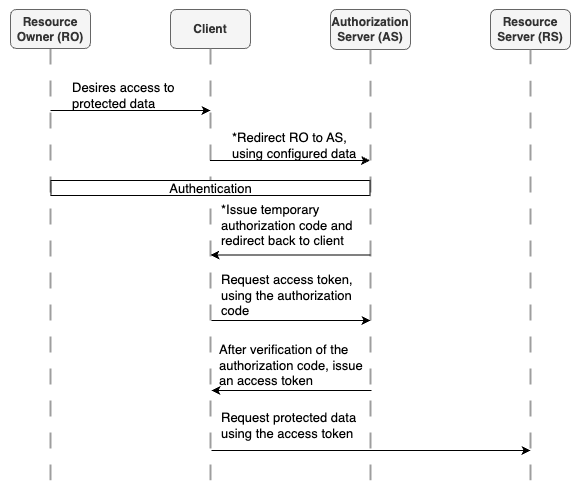
\includegraphics[width=0.6\textwidth]{pic/authorization_code_grant.png}
	\unitlength=0.75mm
	\special{em:linewidth 0.4pt}
	\linethickness{0.4pt}
	\caption{Authorization Code Grant flow without any extensions}
	\label{fig:auth_code_grant}
\end{figure}
	
\begin{itemize}
	\item Implicit Grant
	\item Resource Owner Password Credentials Grant
	\item Client Credentials Grant
	\item Refresh Token Grant
	\item JWT Bearer Grant
	\item Device Code Grant
	\item UMA Grant
	\item SAML 2.0 Bearer Grant
	\item Token Exchange Grant
\end{itemize}
\todo{Decide on how to handle niche grant types}

\subsection{OpenID}

\subsection{The Future: OAuth 2.1}

\section{Intrusion Detection}

\subsection{zeek IDS}

\section{Algorithms}

\chapter{Literature Study: Taxonomy of OAuth Vulnerabilities}
\section{OAuth Vulnerabilities}

\subsection{Insufficient Redirect URI Validation \cite{lodderstedt2020oauth} \cite{wang2019make}}
Authorization Servers need to whitelist redirection URLs in order to make sure, that an attacker cannot craft a hyperlink, which leads to the victim initiating an OAuth flow and sending the authorization code or token to an attacker-controlled domain. Some authorization servers may allow the usage of patterns in order to allow several domains at once. As well as the absence of any sort of whitelist mechanism even a pattern-matching functionality could lead to security problems. Among the possibility that a user is entering patterns that are too broad and allow the usage of unintended redirect URLs, the attack surface includes issues with the URL parsing implemented by the authorization server as shown by Wang et al. \cite{wang2019make}. They presented several techniques to trick the parser into accepting unintended domain names, like using squared brackets for IPv6 parsing or the \emph{Evil Slash Trick}, where the parser does not treat a forward slash as a path separator, while modern browsers do. Depending on the OAuth grant type in use this vulnerability leads to different possibilities to exploit it.


\subsubsection{Authorization Code Flow}
\begin{itemize}
	\item The attacker uses techniques like phishing to make its victim open an attacker-controlled webpage, which initiates an OAuth flow with the vulnerable authorization server.
	\item The request is crafted with a valid client ID (which is public information), ``code'' as response type and a malicious redirect URI, which leads to an attacker-controlled server again.
	\item If the user logs in at the authorization server, the authorization code now gets transmitted to the attacker's webpage, via the redirect URI.
	\item The attacker page can now use the received authorization code, to retrieve a token 
\end{itemize}

\subsubsection{Implicit Flow}
\todo{Maybe write down open redirection with the implicit flow here regarding redirect\_uri check circumvention}


\subsection{Credential Leakage via Referer Headers}
The Referer HTTP header is a potential attack surface. It can be utilized by a malicious actor to capture query parameters, which are sent via the front channel, like the state and the authorization code. The authorization code may be used to redeem an access token before the victim retrieves it and the state parameter oftentimes includes a CSRF token, which could potentially open up vulnerabilities in other parts of the application as explained by Fett et al \cite{fett2016comprehensive}.

\subsubsection{OAuth Client}
If a client renders third-party content, like advertisements in iframes or images, before redeeming the authorization code for an access token an attacker, who places these advertisements or images can capture the code via the referer header and redeem it for an access token.

\subsubsection{Authorization Server}
At the authorization server, the state parameter could be leaked via the Referer header, when 3rd party images or advertisements are being rendered on the page. This may be an issue when the state contains a CSRF token as explained by Fett at al \cite{fett2016comprehensive}.


\subsection{Credential Leakage via Browser History}
\todo{Find studies about risks of confidential data in browser history} 

\subsection{Mix-Up Attacks}

\subsection{Authorization Code Injection \cite{philippaerts2022oauch}} 
The precondition for an authorization code injection is that an attacker has successfully stolen an authorization code. This can be accomplished in various ways for example by tricking the user into installing a malicious browser extension, using other vulnerabilities in a web app like open redirections, or abusing proxy auto-configuration files \cite*{philippaerts2022oauch}.

In the case, that the client is using the authorization code flow the attacker can use the stolen authorization code to fetch an access token before the client does.

\subsection{Countermeasures}
There are several ways to mitigate the risk of authorization code injection. For example, if an authorization code got used twice in the case it got stolen and the attacker, as well as the client, tried to redeem a token, every token that was redeemed with this authorization code should get invalidated. Another method is the usage of PKCE to make sure the OAuth flow is only used, between the two legitimate parties.



\subsection{Access Token Injection}

\subsection{Cross Site Request Forgery}
This type of attack, often referred to by its abbreviation ``CSRF"", is about the attacker executing a request in the name of the user, by tricking the user into executing requests for the attacker including all required authentication, or authorization information. The default OAuth protocol does not include protection mechanisms against this type of attack. 

\subsection{PKCE Downgrade Attacks}

\subsection{Access Token Leakage at the Ressource Server}

\subsection{Misuse of Stolen Access Tokens}

\subsection{Open Redirection}

\subsection{307 Redirect}

\subsection{TLS Terminating Reverse Proxies}

\subsection{Refresh Token Protection}

\subsection{Client Impersonating Resource Owner}

\subsection{Clickjacking}

\subsection{Authorization Server Redirecting to Phishing Site}

\subsection{Attacks on In-Browser Communication Flows}

\section{Countermeasures}
\subsection{PKCE system}
As an extension to OAuth defined by RFC 7636, ```Proof Key for Code Exchange'' is a technique to mitigate Authorization Code Injection misuse or CSRF attacks \cite{bradley2015rfc}. Specifically, it extends the authorization code flow 

\chapter{Intrusion Detection: State of the Art}

\chapter{Algorithmic Approach}

\chapter{Experimental Analysis}

\chapter{Conclusion}


% =============================Literaturverzeichnis=============================
\begin{raggedright}         % Schaltet Blocksatz ab, erzeugt ein stimmigeres
                            %  Schriftbild im Literaturverzeichnis.
  \printbibliography        % Falls Biblatex verwendet wird.
  \label{sec:literaturverzeichnis}
\end{raggedright}


% ===================================Anhang=====================================
\appendix
\setcounter{figure}{0}
\renewcommand\thetable{A.\arabic{figure}}
\setcounter{table}{0}
\renewcommand\thetable{A.\arabic{table}}
% ===========================Selbstständigkeitserklärung======================
\chapter*{Eidesstattliche Versicherung} % war: Selbständigkeitserklärung
\vspace{1cm}

\todo[noline]{Bitte verwenden Sie hier in jedem Fall die offizielle von der Prüfungsbehörde vorgegebene Formulierung der Selbständigkeitserklärung.}
%
Hiermit versichere ich an Eides statt, dass ich die vorliegende Arbeit selbstständig verfasst und keine anderen als die angegebenen Hilfsmittel – insbesondere keine im Quellenverzeichnis nicht benannten Internet-Quellen – benutzt habe. Alle Stellen, die wörtlich oder sinngemäß aus Veröffentlichungen entnommen wurden, sind als solche kenntlich gemacht. Ich versichere weiterhin, dass ich die Arbeit vorher nicht in einem anderen Prüfungsverfahren eingereicht habe und die eingereichte schriftliche Fassung der auf dem elektronischen Speichermedium entspricht.

Ggf. streichen: Ich bin damit einverstanden, dass meine Abschlussarbeit in den Bestand der Fachbereichsbibliothek eingestellt wird.

\makeatletter
Hamburg, den {\@date}
\makeatother

\vspace{2cm}
\rule{6cm}{0.25pt}\\
\makeatletter
{\@author} \par
\makeatother




% ================================Literaturliste-Muster==============================
\newpage
\thispagestyle{empty}
\label{sec:literaturliste}
\par\textbf{\textsf{Thema:}} Privacy Enhancing Technologies zum Schutz von Kommunikationsbeziehungen
\par\textbf{\textsf{Bearbeiter:}} Eva Musterfrau, Heinz Mustermann
\par\textbf{\textsf{Datum:}} \today
\bigskip
% ====> Delete me
\begin{tikzpicture}[overlay]
    \node[draw, blue, font=\sffamily\Large, xshift=70mm, yshift=0mm, rounded corners=1mm]{Muster der Literaturliste};
\end{tikzpicture}
% <==== /Delete me
\par\textbf{\Large\textsf{Literaturliste}}

% ================================Todo list==============================
\listoftodos
% \todototoc

\end{document}
